\subsection{Syntax-number units interactions}[t]
\begin{figure*}
\centering
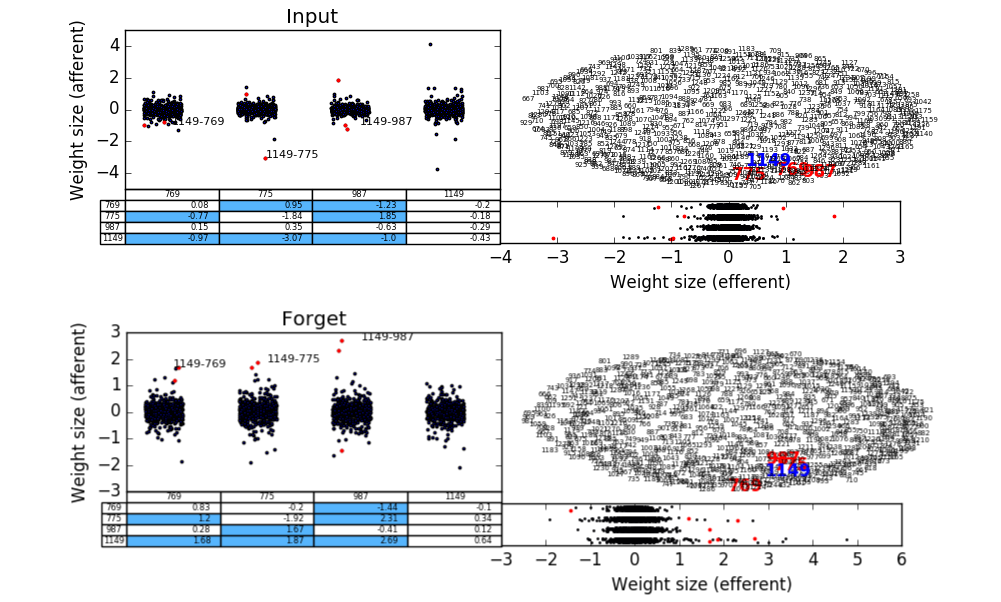
\includegraphics[width=\textwidth]{Figures/Figure7_interactions.png}
\caption{Interaction among the syntax and number units. A value in the table represents the weight size from the unit appearing on the left to the unit appearing on the top row. (A) Distribution of all weight values to the unit appearing on the top row of the table. Outlier weights from the table (more than three standard-deviation above/below the mean) are marked in red; Weight values from the syntax to number units have in addition a corresponding text label. (B) Distribution of all weight values from the unit appearing on the left column of the table. Outlier weights are marked in red. (C)  A visualization of unit interactions. For each gate $g$, an interaction distance $d_{ij}^g$ between a pair of units $i$ and $j$ was first defined as: $d_{ij}^g=exp{-max{w_{ij}^g, w_{ji}^g}}$, where $w_{ij}^g$ is the weight from unit $j$ to the gate $g$ of unit $i$. Then, all interaction distances in the network were visualized using multidimensional scaling. Note that the interaction distances between the number units and between the syntax and number units are relatively close compared to the mean interaction distance in the network.}
\end{figure*}

In the previous sections, it was shown that units 988 and 776 carry singular and plural number inofmation across long-range dependecies, and that in various sentences hidden-state activity of unit 1150 follows the structure of the phrase embedded betweent the main subject and verb. As discussed, both types of information, number and syntactic structure, seem required for accompolishing the NA-task. Moreover, to time the storage and update of number information, we expected that the activity of the LR number units be controlled and affected by the activity of the syntax units, and in particular by that of unit 1150. To explore this, we now look into the connectivity of the network, focusing on the connection weights among these units. We note that for each pair of units that are four types of connection corresponding to the four types of gates: suggestion, input, forget and output gates.

Figure X shows the distribution of all afferent (top-left) and efferent (bottom-right) recurrent weights of units 776 988 and 1150 for both input and forget gates (panel A\&B). In addition, all weight values among these three units (also represented as red dots in panels A and D). 
